%%%%%%%%%%%%%%%%%%%%%%%%%%%%%%%%%%%%%%%%%
% Short Sectioned Assignment
% LaTeX Template
% Version 1.0 (5/5/12)
%
% This template has been downloaded from:
% http://www.LaTeXTemplates.com
%
% Original author:
% Frits Wenneker (http://www.howtotex.com)
%
% License:
% CC BY-NC-SA 3.0 (http://creativecommons.org/licenses/by-nc-sa/3.0/)
%
%%%%%%%%%%%%%%%%%%%%%%%%%%%%%%%%%%%%%%%%%

%----------------------------------------------------------------------------------------
%	PACKAGES AND OTHER DOCUMENT CONFIGURATIONS
%----------------------------------------------------------------------------------------

\documentclass[paper=a4, fontsize=11pt]{scrartcl} % A4 paper and 11pt font size

\usepackage[T1]{fontenc} % Use 8-bit encoding that has 256 glyphs
\usepackage{fourier} % Use the Adobe Utopia font for the document - comment this line to return to the LaTeX default
\usepackage[english]{babel} % English language/hyphenation
\usepackage{amsmath,amsfonts,amsthm} % Math packages
\usepackage{url}

\usepackage{graphicx}
\usepackage{hyperref}
\usepackage{subfigure}
\usepackage{lipsum} % Used for inserting dummy 'Lorem ipsum' text into the template

\usepackage{sectsty} % Allows customizing section commands
\allsectionsfont{\centering \normalfont\scshape} % Make all sections centered, the default font and small caps

\usepackage{fancyhdr} % Custom headers and footers
\pagestyle{fancyplain} % Makes all pages in the document conform to the custom headers and footers
\fancyhead{} % No page header - if you want one, create it in the same way as the footers below
\fancyfoot[L]{} % Empty left footer
\fancyfoot[C]{} % Empty center footer
\fancyfoot[R]{\thepage} % Page numbering for right footer
\renewcommand{\headrulewidth}{0pt} % Remove header underlines
\renewcommand{\footrulewidth}{0pt} % Remove footer underlines
\setlength{\headheight}{13.6pt} % Customize the height of the header

\numberwithin{equation}{section} % Number equations within sections (i.e. 1.1, 1.2, 2.1, 2.2 instead of 1, 2, 3, 4)
\numberwithin{figure}{section} % Number figures within sections (i.e. 1.1, 1.2, 2.1, 2.2 instead of 1, 2, 3, 4)
\numberwithin{table}{section} % Number tables within sections (i.e. 1.1, 1.2, 2.1, 2.2 instead of 1, 2, 3, 4)

\setlength\parindent{0pt} % Removes all indentation from paragraphs - comment this line for an assignment with lots of text

%----------------------------------------------------------------------------------------
%	TITLE SECTION
%----------------------------------------------------------------------------------------

\newcommand{\horrule}[1]{\rule{\linewidth}{#1}} % Create horizontal rule command with 1 argument of height

\title{	
\normalfont \normalsize 
\textsc{University of Bucharest, College of Mathematics and Computer Science  } \\ [25pt] % Your university, school and/or department name(s)
\horrule{0.5pt} \\[0.4cm] % Thin top horizontal rule
\huge Substitution matrices \\ % The assignment title
\horrule{2pt} \\[0.5cm] % Thick bottom horizontal rule
}

\author{\c Stefan Cobeli} % Your name

\date{\normalsize\today} % Today's date or a custom date

\begin{document}

\maketitle % Print the title

%----------------------------------------------------------------------------------------
%	PROBLEM 1
%----------------------------------------------------------------------------------------

\section{Substitution matrix}

\lipsum[200]  %Dummy text

\paragraph{}PAM is the abreviation for \textit{Point Accepted Mutation} and it's a type of substitution matrix. The PAM1 matrix is instantiate by a \textit{ Log Odds } table and  generates all the other PAM matrices by multiplication.\\
The original name of this matrix was Accepted point mutation, but APM is much harder to pronounce than PAM, so Margaret Dayhoff chosen the second alternative.

%------------------------------------------------

\paragraph{PAM1 construction}
If we have \textit{n} proteins and we want to construct their PAM1 matrix, we give them an order. The position \textit{i,j} of the matrix will be populated with the value of probability that the protein \textit{i} mutates to protein \textit{j} after \textit{1\%} of it's changed.


\begin{figure}[h!]
  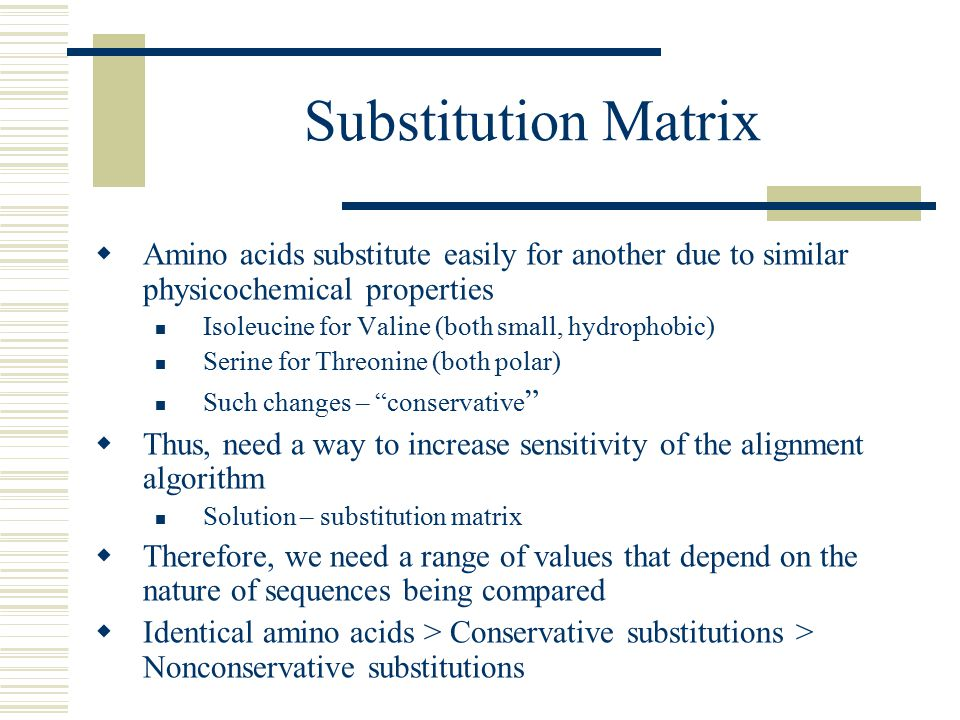
\includegraphics[width=\linewidth]{About_substitution_matrix1.jpg}
 	This is a description of substitution matrices. If it looks interesting, here is some more:
 	\cite{Sub1}.
  \label{fig:boat1}
\end{figure}
\newpage



\begin{figure}[h!]
  
\includegraphics[width=\linewidth]{shiny_BLOSUM.png}
 	BLOSUM is a type of substitution matrix. 
  \label{fig:boat1}
\end{figure}
\newpage

\begin{figure}
\hfill
\subfigure[Place \cite{Sub2}]{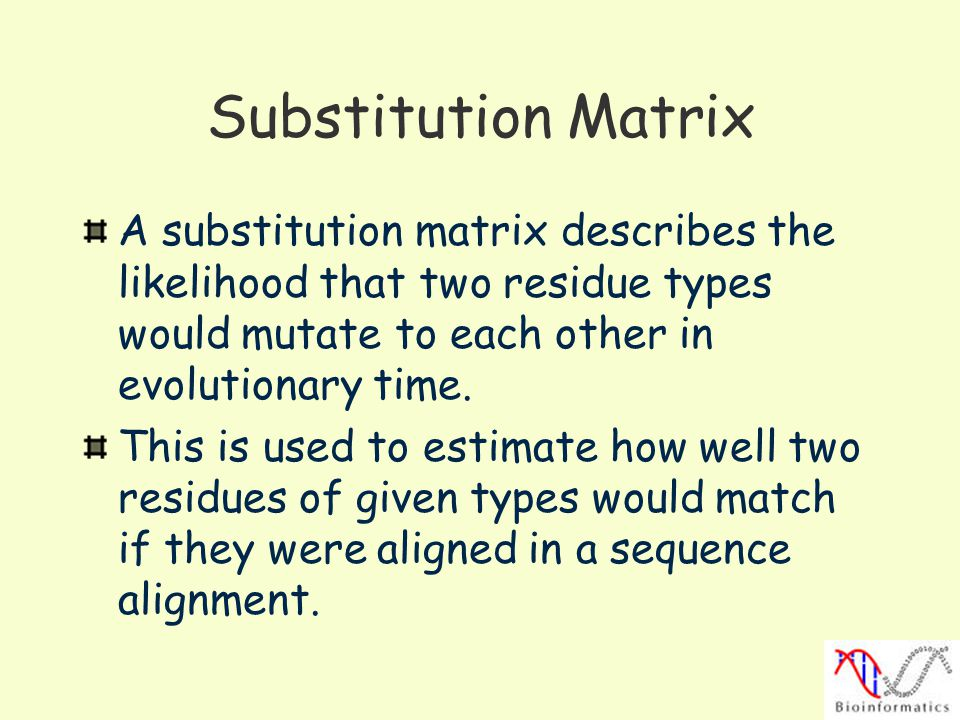
\includegraphics[width=5cm]{About_substitution_matrix2.jpg}}
\hfill
\subfigure[Place \cite{Sub3}]{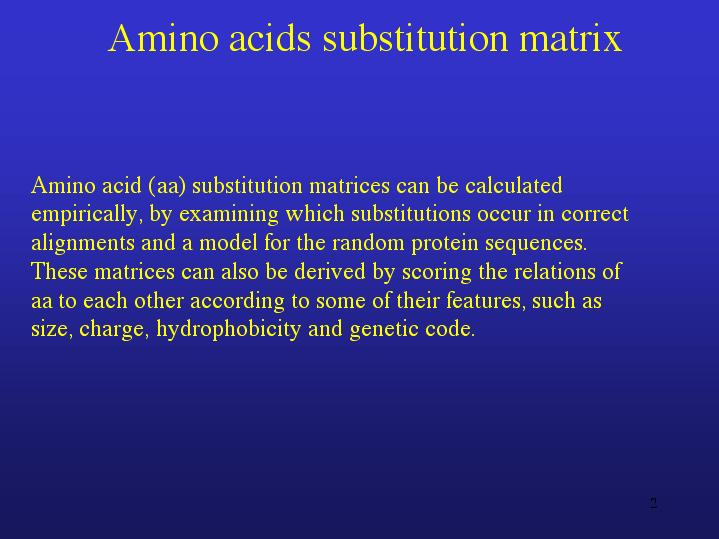
\includegraphics[width=5cm]{About_substitution_matrix3.jpg}}
\hfill
\caption{Here are two more places from which you can also read about substitution matrices}
\end{figure}




%------------------------------------------------

\newpage
%----------------------------------------------------------------------------------------
%	PROBLEM 2
%----------------------------------------------------------------------------------------
\newpage
\section{Etics}

%------------------------------------------------


Here we have an extract from the \textit{Etics Rules} from the \textit{Faculty of Mathematics and Computer Science} of \textit{University of Bucharest}. \cite{Etica}

\begin{quote}

REGULAMENT DE ETICĂ ȘI PROFESIONALISM
PENTRU FACULTATEA DE MATEMATICĂ ȘI INFORMATICĂ (FMI)
A UNIVERSITĂȚII DIN BUCUREȘTI
Interacțiunea profesor - student presupune, pe lângă respectul reciproc, și alte aspecte
ce trebuie avute în vedere pentru menținerea unui cadru civilizat și plăcut pe parcursul
desfășurării activităților didactice.
Regulamentul de etică și profesionalism pentru FMI se dorește a fi un îndrumător pentru
ambele părți implicate în procesul de învățământ (profesori și studenți), în vederea
creării unui astfel de cadru. Regulamentul exemplifică situații ce se doresc a fi evitate și
normează modul în care se va acționa în cazul unor conflicte de natură etică.
Principii generale
1. Cadrele didactice și studenții FMI se vor comporta într-o manieră etică, atât în cadrul
facultății, cât și în afara ei.
2. Cadrele didactice ale FMI îi vor îndruma pe studenți spre o conduită etică și
profesională.
3. Se va folosi prezumția de nevinovăție, orice incident raportat va trebui probat.
4. Persoanele implicate într-un incident de etică vor avea dreptul de a se apăra.
5. Acest regulament este adoptat cu scopul de a ajuta Facultatea să-și păstreze
renumele și, implicit, îi ajută pe studenții care obțin o diplomă de la FMI.
6. Regulamentul nu are un rol coercitiv, ci un rol corector.
7. În acest regulament vom considera doua tipuri de incidente: incidente minore (care
se pot justifica prin necunoașterea unor reguli de etică și profesionalism) și incidente
majore (care sunt determinate de o acțiune voluntară).
Articole
1. Considerând principiile de mai sus, cadrele didactice și studenții care observă o
încălcare a eticii în Facultate vor raporta în scris incidentul la secretarul șef al FMI.
Raportul va descrie fapta, va conține numele și semnătura raportorului, precum și
numele a încă două persoane care au fost de față și/ sau probe și dovezi materiale.
2. Incidentul astfel raportat va primi un număr de înregistrare la secretariat. În cazul în
care incidentul este raportat de către un cadru didactic, acesta va cataloga incidentul
în incident minor sau incident major.
3. Orice raportare a unui incident în care este implicat un student/ o studentă va fi
adusă la cunoștință persoanei respective de către secretariat. Studentul/ studenta va
putea primi o copie a raportului (fără semnături sau date de identificare ale martorilor)
și va avea o perioadă de 5 zile lucratoare în care să poată depune o cerere pentru
constituirea unei comisii de etică pentru evaluarea cazului.
4. Comisia menționată la articolul 3 va fi numită de conducerea Facultății. Comisia va
avea în componență 5 membri: doi studenți și trei cadre didactice. Preferabil,
studenții vor fi din același program de studii ca și studentul incriminat. Cadrele
didactice din comisie vor fi alese din ambele departamente ale Facultății.
5. In cazul in care studentul/ studenta nu depune cererea menționată la articolul 3, sau
în cazul în care comisia de etică constituită conform articolului 3 consideră raportul
întemeiat, respectivul incident va fi înscris într-o bază de date pentru incidentele de
etică. Baza de date va fi completată de către secretarul șef al FMI și va conține
numele studentului/ studentei și detalii privind incidentul raportat (data producerii
incidentului, persoana care a raportat incidentul, numărul de înregistrare al raportului,
tipul de incident, etc.).
6. La acumularea a doua incidente minore, un student va fi consiliat de către un cadru
didactic în ce privește codul de etică al FMI.
7. Comisia menționată la articolul 3 este constituită automat, dacă se raportează un nou
incident minor pentru un student care are deja doua incidente minore, consemnate în
baza de date.
8. Dacă pentru un student, există trei incidente minore sau un incident major,
consemnate în baza de date de la articolul 5, cazul va fi adus la cunoștință Consiliului
Facultății.
9. Consiliul declanșează procedurile care se impun, în conformitate cu regulamentul de
etică al Universitățtii și al Facultății. În cazul în care Consiliul confirmă existența uneia
din situațiile de la art. 8, sancțiunea este exmatricularea. Consiliul decide dacă
studentul/ studenta exmatriculat(ă) are sau nu drept de reînscriere.
10. Niciun cadru didactic (din afara conducerii Facultății) nu va putea consulta baza de
date menționată la art. 5. Informațiile din această bază de date vor fi confidențiale.
11. Exemple de incidente minore în care pot fi implicați studenți.
Se consideră incident minor cazul în care un student/ o studentă:
a. preia codul sursă/ rezolvarea unei teme de la un coleg/ o colegă și pretinde că este
rezultatul efortului propriu;
b. dă unui coleg/ unei colege codul sursă/ rezolvarea unei teme, deja predată;
c. copiază demonstrația unei teoreme/ rezolvarea unei teme cuvânt-cu-cuvânt dintr-o
carte și o prezintă ca fiind a sa, fără indicarea sursei;
d. copiază o temă/ o implementare de laborator din surse publice, fără indicarea sursei;
e. perurbă în mod repetat orele de curs/seminar/laborator;
f. nu respectă un cod minimal de conduită față de colegi și încalcă „bunele moravuri”
(limbajul licențios este o încălcare a bunelor moravuri);
g. are manifestări violente în relație cu colegii și cadrele didactice (violența verbală este
considerată, de regulă, incident minor, iar cea fizică este considerată incident major);
h. inscripționează voluntar bănci sau ziduri din incinta Facultății.
12. Exemple de incidente majore în care pot fi implicați studenți.
Se consideră incident major cazul în care un student/ o studentă:
a. copiază la examene de orice tip;
b. manifestă acte de violență fizică;
c. plagiază la lucrările de licență sau de disertație (preluarea integrală a unui text, chiar
și cu menționarea sursei, preluarea ideilor unui text fără menționarea sursei,
preluarea construcției logice fără menționarea sursei, sunt fapte ce constituie plagiat;
în lucrările de licență sau de disertație, pornim de la premisa că studentul ar trebui să
explice rezultatele teoretice „cu cuvintele sale”, nu să copieze textul dintr-o sursă
bibliografică);
d. distruge cu buna știință obiecte de patrimoniu sau acte oficiale (proiectoare,
calculatoare, lucrări de examen, cataloage);
e. înlocuiește un coleg/ o colegă la un examen;
f. acceptă/ solicită unei alte persoane sa îl/ o înlocuiască la un examen.
13. Regulamentul de față se aplică tuturor studenților FMI, indiferent de programul în
care sunt înmatriculați (licență, master, doctorat).
14. Regulamentul se aplică și studenților care își continuă studiile, după o întrerupere
temporară; în acest caz, se va ține cont de înregistrările din baza de date, anterioare
datei întreruperii studiilor.
15. Orice incident în ce privește etica sau profesionalismul studenților FMI, petrecut în
afara Universității (în firme, instituții publice, etc., în care studentul/ studenta
desfașoară activități organizate de FMI), va activa automat comisia menționată la
articolul 3 și va fi discutat în cadrul comisiei.
16. În cazul dovedirii unei fraude la examenul scris de licență, studentul/ studenta
respectivă va fi eliminat(ă) din examen. Consiliul decide amânarea cu 1 an a
susținerii examenului de licență. Incidentul va fi înscris în baza de date menționată la
art. 5.
17. Cadrele didactice au datoria de a raporta incidentele care apar în timpul desfășurării
activităților didactice. Spre exemplu, dacă un student este penalizat prin notă pentru
plagiere/ copiere a unei teme, automat profesorul va raporta incidentul respectiv.
18. Orice incident de etică referitor la cadre didactice, raportat de alte cadre didactice
sau de studenți, se aduce obligatoriu la cunoștința Consiliului Facultății. Consiliul
poate decide înființarea unei comisii de etică pentru evaluarea cazului. În această
situație, comisia prezinta Consiliului un raport: dacă acesta este considerat întemeiat,
conducerea Facultății va sesiza Comisia de Etică a Universității din București. 

\end{quote}


\newpage
\paragraph{}
\begin{figure}[h!]
  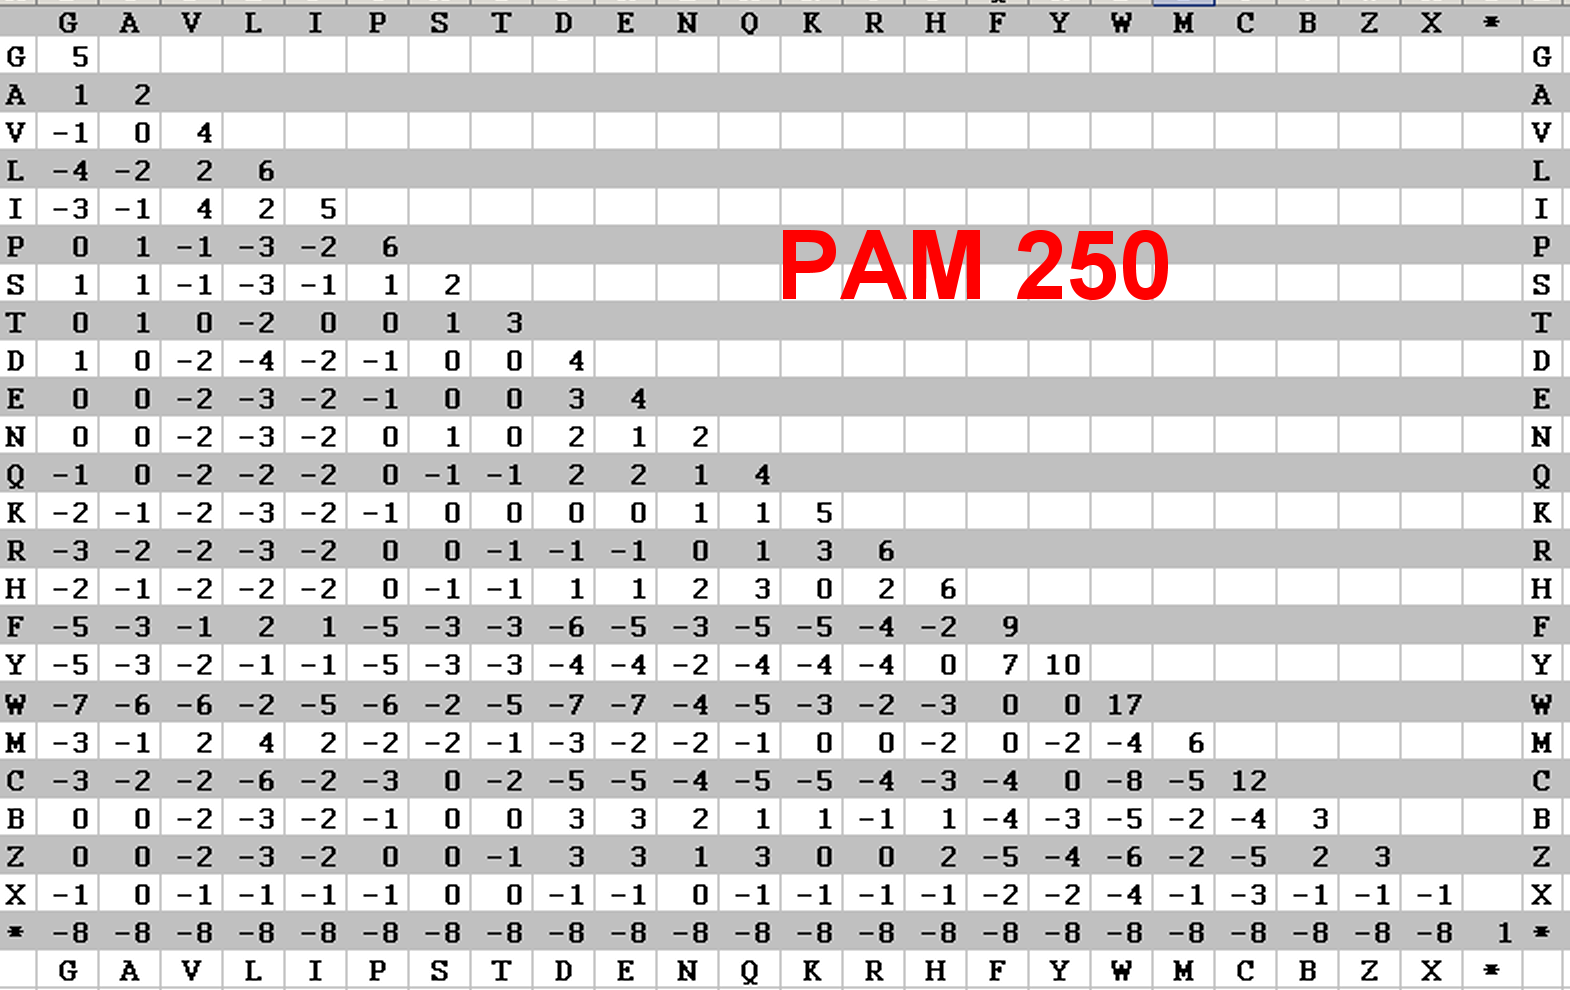
\includegraphics[width=\linewidth]{pam250.png}
 	This is an example of a PAM matrix, which is also a substitution matrix.
  \label{fig:boat1}
\end{figure}

\newpage
{\small
\begin{thebibliography}{9999}

\bibitem{Sub1}
\url {http://slideplayer.com/slide/5229054/}\\

\bibitem{Sub2}
\url {http://slideplayer.com/slide/1661678/}\\

\bibitem{Sub3}
\url {http://bip.weizmann.ac.il/education/course/ATIB/ATIB02/lecture3/sld001.htm}\\

\bibitem{Etica}
\url {http://fmi.unibuc.ro/ro/pdf/2015/consiliu/Regulament_etica_FMI.pdf}\\


\end{thebibliography}
}

%------------------------------------------------


%----------------------------------------------------------------------------------------

\end{document}